\documentclass[11pt]{article}

% "review" for submission (anonymous, line numbers); "final" for camera-ready; "preprint" for arXiv.
\usepackage[review]{acl}

\usepackage{times}
\usepackage{latexsym}
\usepackage[T1]{fontenc}
\usepackage[utf8]{inputenc}
\usepackage{microtype}
\usepackage{inconsolata}
\usepackage{graphicx}
\usepackage{booktabs}
\usepackage{amsmath}
\usepackage{xcolor}

% Drafting marks: remove before submission.
\newcommand{\todo}[1]{\textcolor{red}{[TODO: #1]}}

\title{Judges Approve What They Believe:\\Belief, Not Authorship, Drives LLM Judges' Approval of Wrong Answers}

\author{Anonymous ACL submission}

\begin{document}
\maketitle

% ---------------------------------------------------------------------------------------------------------------
\begin{abstract}
LLM judges approve wrong answers, and prior work attributes part of this to self-preference: judges favour text
they wrote. We separate authorship from belief. For every candidate answer, written by a \emph{different} model,
we measure the judge's belief as the share of its own seven independent solutions that reach the same final
answer. Across four benchmarks and six judges from four model families, approval of wrong answers rises steadily
with belief: from 17\% when the judge never reaches the answer to 65\% when it always does (three Qwen judges;
Nemotron-3-Super 26\%$\rightarrow$88\%, DeepSeek-V4.1-Flash 13\%$\rightarrow$55\%, Kimi-K2.6 2\%$\rightarrow$65\%),
and the rise survives a full audit of the benchmark labels. Belief explains away the usual one-sample ``matches my answer'' signal, and the same
wrong answer is approved more by the judge that believes it more. Transcripts show judges re-solving the problem and
approving when they land on the candidate's answer. Inside the model, read before any verdict is generated, the
direction separating believed from never-reached wrong answers aligns with the judge's correctness direction
(cosine 0.70--0.80) far more than it does while the model solves (0.25--0.36). The audit also shows that a
``wrong'' answer that judges strongly believe is often a label error: 23 of 55 such answers are actually correct.
\end{abstract}

% ---------------------------------------------------------------------------------------------------------------
\section{Introduction}

LLM-as-a-judge is now the default way to score open-ended outputs, to build preference data and to run
benchmarks \citep{zheng2023judging}. Its best-known failure is self-preference: judges rate their own generations
higher \citep{panickssery2024llm}. Two recent results suggest a different reading. Much of what looks like
self-preference is the judge being wrong about the question \citep{roytburg2026narcissists}, and judges agree with
human experts mainly on questions they can answer themselves \citep{krumdick2026nofreelabels}. Both point to the
judge's own \emph{answer}, not its authorship, as the thing that matters.

We test this directly and per answer. A judge grades candidate answers written by other models, so authorship is
removed by construction. Separately, and without ever seeing the candidate, the judge solves the same question
seven times. Its \emph{belief} in a candidate is the share of those solutions that reach the candidate's final
answer, from 0/7 to 7/7. We then ask three questions:
\begin{enumerate}
\item Does a judge approve wrong answers more the more strongly it believes them?
\item How does it get there: what do judges write before approving?
\item What happens inside the model while it judges?
\end{enumerate}

\paragraph{Contributions.}
\begin{itemize}
\item \textbf{A belief staircase.} Approval of wrong answers rises monotonically with belief in six judges from
four families (Figure~\ref{fig:staircase}), on audited labels. Belief accounts for the effect of the usual
one-sample ``matches my answer'' label, and the same wrong answer is approved more by the judge that believes it more
(+23 points), which authorship cannot explain.
\item \textbf{A mechanism.} Judges re-solve and check for a match: with reasoning visible, 92--100\% of approved
wrong answers come with a re-solve that lands on the same wrong answer. Inside the model, while judging, believing a
wrong answer looks like it being right (cosine 0.70--0.80 between the belief and correctness directions, against
0.25--0.36 while solving), and this survives removing the model's lean toward saying CORRECT.
\item \textbf{A label audit.} Label errors concentrate exactly where judges believe the answer: 23 of 55 ``wrong''
answers believed 7/7 are correct, against 2 of 245 at 0/7. Released labels therefore inflate the top of the
staircase; we report every result on audited labels.
\end{itemize}

% ---------------------------------------------------------------------------------------------------------------
\section{Related Work}

\paragraph{Judges and their own answers.}
\citet{panickssery2024llm} show that judges recognise and prefer their own generations. \citet{roytburg2026narcissists}
argue that much of this preference is the judge being wrong on the question; we measure that belief per answer and
remove authorship entirely. \citet{krumdick2026nofreelabels} find that judges agree with experts mainly on questions
they can answer, and that expert references largely fix this; we grade the same phenomenon per answer, on a 0--7
scale, and use their BFF-Bench data. \citet{goel2025great} show that judges favour models that make the same
mistakes; ours is the per-answer version of this model-level effect. \citet{lin-etal-2025-before} find that solving
and judging ability are only weakly correlated, and that the judge's own answer as a reference strengthens the link;
we test this ``commit first'' prompt by belief level (\S\ref{sec:juries}).

\paragraph{Truth and belief inside models.}
Linear directions separate true from false statements in hidden states \citep{marks2024geometry,burns2023discovering,
azaria-mitchell-2023-internal}, and difference-of-means directions can steer behaviour
\citep{rimsky-etal-2024-steering,arditi2024refusal,zou2023representation}. Whether such probes read truth or the
model's belief is contested \citep{herrmann2025standards}: a ``correctness'' probe behaves like the model's belief
\citep{yang2026admit}, output confidence tracks belief rather than truth \citep{cho2026confidence}, and on judges,
correctness labels cannot separate truth from the judge's belief \citep{gulati2026auditing}.
\citet{mukherjee2026opening} find that judges' activations often hold the right preference when the verdict is
wrong. We build belief and correctness as two separate directions, belief from wrong answers only, and compare them
while the same model judges and while it solves.

% ---------------------------------------------------------------------------------------------------------------
\section{Measuring Belief}
\label{sec:setup}

\paragraph{Benchmarks.}
Every item is a question, one candidate answer written by another model, and a right/wrong label.
\textbf{RewardBench~2 Math} \citep{malik2025rewardbench2}: 183 questions, 732 single answers, short final values.
\textbf{JudgeBench} \citep{tan2025judgebench}: 547 response pairs with letter answers (coding pairs dropped), where
the judge picks the better response. \textbf{BFF-Bench} \citep{krumdick2026nofreelabels}: 459 answers to
finance questions with unanimous expert labels, single- and two-turn. \textbf{BBEH}
\citep{kazemi-etal-2025-big}: about 2,000 answers to hard reasoning puzzles, used for the inside-the-model analysis.

\paragraph{Judges.}
Qwen3.5-4B, Qwen3.5-9B and Qwen3.6-35B-A3B (Alibaba); Nemotron-3-Super-120B-A12B (NVIDIA); DeepSeek-V4.1-Flash
(DeepSeek); and Kimi-K2.6 (Moonshot). All judge with thinking off: the model writes a short justification and
ends with a verdict line. The judge never wrote any of the candidates it grades.

\paragraph{Belief.}
For each question the judge answers seven more times at temperature 0.7, with only the question (and, for
two-turn BFF items, the earlier turns) in context. Belief in a candidate is the number of these seven answers that
reach the candidate's final answer, divided by seven. A separate, eighth answer defines the one-sample
``matches my answer'' label used in prior work, so the two are independent measurements. JudgeBench letters are
matched exactly. On RewardBench~2 Math and BFF-Bench, GLM-5.3-Flash, a model from a family none of the judges
belongs to, decides whether two final answers are the same, ignoring wording and rounding
(Appendix~\ref{app:matcher}). A second reader agreed with 42 of 47 of its decisions on a stratified sample; every
disagreement was the matcher saying DIFFERENT on a near-match, so belief is, if anything, understated.

\paragraph{Label audit.}
A ``wrong'' answer that a judge reaches in all seven tries is either a confident error or a label error. We audited
every wrong-labelled answer. On RewardBench~2 Math, GLM-5.3-Flash compared each wrong answer's final value with each
right answer to the same question (61 answers removed). On BFF-Bench and JudgeBench, GLM-5.3 audited all 452
wrong-labelled answers against the question, the expert reference or gold option, and its own working, as
\emph{clearly wrong}, \emph{actually correct} or \emph{contested}; a second reader (Claude) read the 55 believed 7/7,
making the same clearly-wrong-or-not call as GLM-5.3 on 87\% of them. Table~\ref{tab:audit} shows the result: label errors
concentrate where judges believe. One example: a BFF-Bench reference copies the question's \$386{,}000 fair value as
\$368{,}000. Unless stated otherwise, every number below uses only answers audited as clearly wrong.

\begin{table}[t]
\centering
\small
\resizebox{\columnwidth}{!}{%
\begin{tabular}{lrrr}
\toprule
Belief & Clearly wrong & Actually correct & Contested \\
\midrule
0/7 & 233 & 2 & 10 \\
1--3 & 120 & 15 & 18 \\
4--6 & 57 & 23 & 21 \\
7/7 & 23 & 23 & 9 \\
\bottomrule
\end{tabular}}
\caption{Audit of wrong-labelled BFF-Bench and JudgeBench answers (unique answers), by the highest belief any Qwen
judge has in them. Judges approve the actually-correct ones 59--82\% of the time.}
\label{tab:audit}
\end{table}

% ---------------------------------------------------------------------------------------------------------------
\section{Approval Rises with Belief}
\label{sec:staircase}

\begin{figure}[t]
\centering
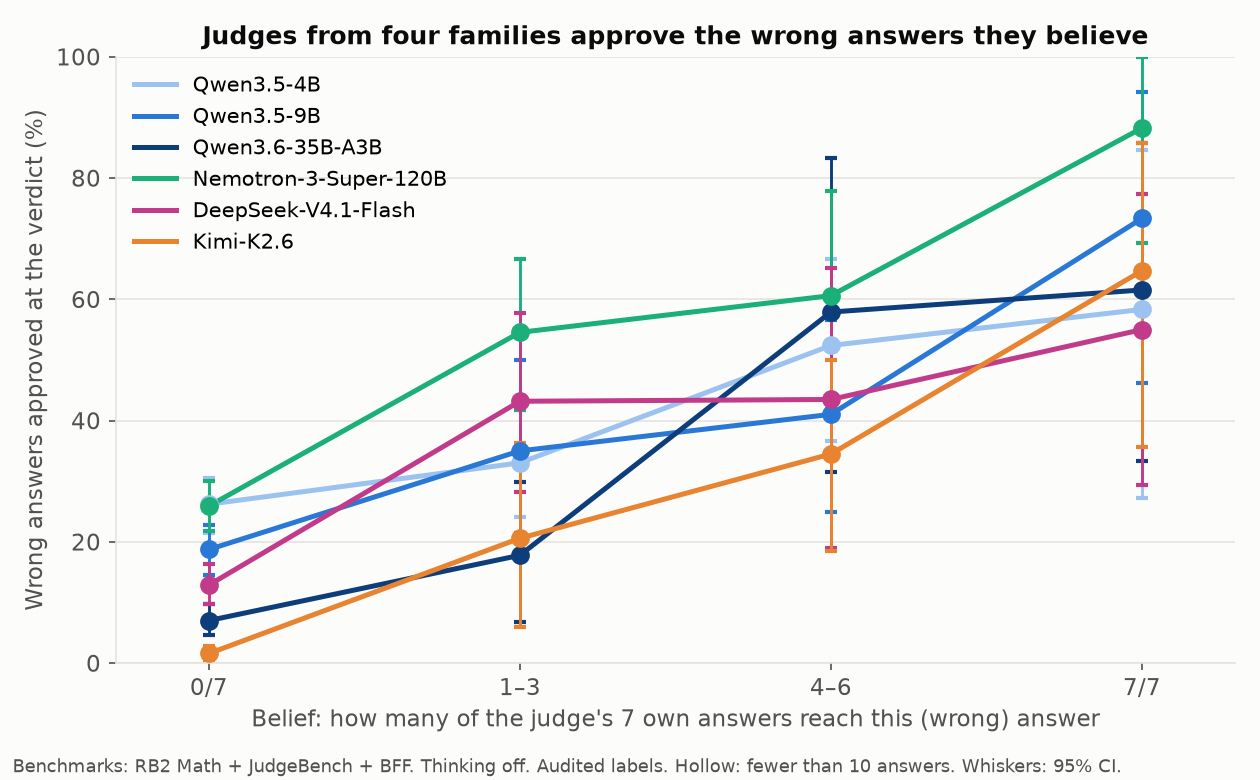
\includegraphics[width=\columnwidth]{figures/staircase.png}
\caption{Wrong answers approved, by the judge's belief in them (RewardBench~2 Math, JudgeBench, BFF-Bench; audited
labels; thinking off). Whiskers: 95\% intervals resampling questions.}
\label{fig:staircase}
\end{figure}

Figure~\ref{fig:staircase} and Table~\ref{tab:families} show the main result. When a judge never reaches a wrong
answer itself (0/7), it approves it 2--26\% of the time depending on the judge. When it always reaches it (7/7), it
approves it 55--88\% of the time. The rise is steady across the intermediate levels and appears in every family.
The released labels exaggerate it at the top (Qwens 18\%$\rightarrow$74\%), because many believed ``wrong'' answers
are right, but cleaning only shrinks the gap (+56 to +48 points for the Qwens).

\begin{table}[t]
\centering
\small
\setlength{\tabcolsep}{4pt}
\resizebox{\columnwidth}{!}{%
\begin{tabular}{lrrrrr}
\toprule
Judge & 0/7 & 1--3 & 4--6 & 7/7 & Gap \\
\midrule
3 Qwens & 17 & 30 & 49 & 65 & +48 {\scriptsize[+30, +63]} \\
Nemotron-3-Super & 26 & 55 & 62 & 88 & +62 {\scriptsize[+45, +76]} \\
DeepSeek-V4.1-Flash & 13 & 42 & 43 & 55 & +42 {\scriptsize[+20, +65]} \\
Kimi-K2.6 & 2 & 21 & 34 & 65 & +63 {\scriptsize[+40, +85]} \\
\bottomrule
\end{tabular}}
\caption{Wrong answers approved (\%), by belief, audited labels. Gap: 7/7 minus 0/7 in points, with a 95\% interval
resampling answers. At 7/7 the groups hold 40, 17, 20 and 17 answers.}
\label{tab:families}
\end{table}

\paragraph{Belief, not a single sample.}
Prior work compares a candidate with one answer from the judge. Fitting both in one model with judge fixed effects,
the Qwens' approval rises by +54 points [+45, +63] from belief 0/7 to 7/7; holding belief fixed, the one-sample
label adds +3 [$-$6, +12], while holding the label fixed, belief adds +52 [+39, +63]. Nemotron (+2 vs +48),
DeepSeek ($-$14 vs +69) and Kimi ($-$0 vs +57) show the same pattern. The one-sample label is a noisy proxy for belief.

\paragraph{Not authorship.}
No judge wrote any candidate, but a belief every model shares could still be a property of the answer rather than of
the judge. Among wrong answers the three Qwens believe to different degrees, with candidate and judge fixed effects,
the Qwen that believes an answer more approves it more: +23 points [+6, +38] from 0/7 to 7/7.

\paragraph{Where the effect forms.}
Reading the verdict a judge would give before it writes anything (by appending ``VERDICT:'' and comparing the
probabilities of the two verdict words) already shows +35 points; the written justification raises it to +54. A
larger Qwen is stricter on answers it does not believe (27\%$\rightarrow$8\% at 0/7, as released) but just as
trusting of answers it does.

% ---------------------------------------------------------------------------------------------------------------
\section{How Judges Approve: Transcripts}
\label{sec:transcripts}

GLM-5.3-Flash labelled 7,443 judging transcripts from the three Qwens: does the judge work out its own answer, and
does that answer equal the candidate's? Eight labels were checked by hand. Among approved wrong answers (ranges over
belief levels):

\begin{center}
\small
\resizebox{\columnwidth}{!}{%
\begin{tabular}{lcc}
\toprule
& Thinking off & Thinking on \\
\midrule
Re-solves the problem & 26--44\% & 92--100\% \\
\quad and lands on the candidate's answer & 23--43\% & 86--96\% \\
\bottomrule
\end{tabular}}
\end{center}

With reasoning visible, approving a wrong answer almost always means re-solving the problem and arriving at that
same answer. Rejections also re-solve, but land elsewhere. With thinking off, most approvals (67--86\%) only walk
through the candidate's steps in writing, so the re-solve, if it happens, is not written down. This motivates
looking inside the model.

% ---------------------------------------------------------------------------------------------------------------
\section{Inside the Model}
\label{sec:inside}

\paragraph{Setup.}
For Qwen3.5-9B and Qwen3.6-35B-A3B (thinking off) we place each answer in two roles and read the hidden state at the
last token, with nothing generated. \emph{Judging}: the usual grading prompt, read right after ``VERDICT:''.
\emph{Solving}: the same answer placed in the model's own turn, followed by a neutral request to restate it, read
after ``FINAL:''. In each role we build two difference-of-means directions \citep{marks2024geometry}, after removing
each question's mean: \emph{correctness} (right minus wrong answers) and \emph{belief} (wrong answers believed $\geq$
half the time minus wrong answers never reached; on BBEH, belief comes from five own answers). Belief uses wrong answers only, so it cannot be correctness in
disguise. Directions are built on disjoint halves of the questions, so no answer contributes to both. We use BBEH,
where 122 believed wrong answers per model remain after auditing; the other benchmarks have too few
(Appendix~\ref{app:inside}).

\begin{table}[t]
\centering
\small
\resizebox{\columnwidth}{!}{%
\begin{tabular}{lcc}
\toprule
& Qwen3.5-9B & Qwen3.6-35B \\
\midrule
Belief vs correctness, judging & \textbf{0.70} & \textbf{0.80} \\
\quad with the CORRECT lean removed & 0.84 & 0.93 \\
Belief vs correctness, solving & 0.36 & 0.25 \\
\midrule
Correctness, judging vs solving & 0.05--0.29 & 0.00--0.28 \\
\bottomrule
\end{tabular}}
\caption{Cosines between directions in the hidden state (BBEH, audited labels, best layer per role; two random
directions have cosine $\approx$0.02). Belief and correctness align while judging, much less while solving; the
judge's correctness direction is unrelated to the solver's.}
\label{tab:inside}
\end{table}

\paragraph{Results.}
Table~\ref{tab:inside} shows two findings. First, while judging, the belief direction aligns with the correctness
direction (0.70 and 0.80): a wrong answer the judge believes is represented much like a right answer. While solving,
the same two directions overlap far less (0.36 and 0.25). Second, the judge's correctness direction is nearly
unrelated to the solver's (0.00--0.29 across layers). The judge does not reuse a ready-made sense of ``this is
right''; the two roles connect through the answer itself.

\paragraph{Not just the verdict lean.}
Both directions could partly encode ``about to say CORRECT''. Projecting the model's own CORRECT-vs-INCORRECT verdict
direction out of the hidden states leaves the alignment intact (0.84, 0.93).

\paragraph{Label errors mattered here too.}
Before the audit, BFF-Bench gave 0.80 and 0.49; afterwards it gives 0.43 and 0.11 on only 12--20 believed answers.
Believed ``wrong'' answers that are actually right pull the belief direction toward correctness by construction, so
an unaudited analysis can overstate the alignment.

\paragraph{Steering.}
Adding the belief direction during generation shifts overall leniency (pushing it down lowers approval of right
answers by 7--13 points) but does not selectively remove approvals of believed wrong answers
(Appendix~\ref{app:steering}). We therefore read the alignment as a representation of the match the judge computes,
not as a single control knob.

% ---------------------------------------------------------------------------------------------------------------
\section{Implications for LLM Juries}
\label{sec:juries}

If judges check for a match, errors on answers they do not believe and errors on answers they do believe should
respond to different fixes. Three Qwens, thinking off, as released labels unless stated.

\paragraph{Commit first.}
Placing the judge's own earlier answer in the conversation before it grades removes approvals of wrong answers it
never reaches (0/7: 17\%$\rightarrow$1\%, $-$17 points [$-$20, $-$14]) but barely moves those it always reaches (74\%$\rightarrow$69\%); balanced
accuracy rises from 80\% to 85\%. Shown a wrong answer it does not believe and asked to \emph{solve}, the judge
adopts it only 2\% of the time, so the low-belief approvals come from the grading frame.

\paragraph{A second family.}
Handing believed items to Nemotron lowers balanced accuracy (e.g.\ 86\%$\rightarrow$82\% for Qwen3.6-35B): Nemotron
believes 77--81\% of the same wrong answers. Confident errors are shared across families.

\paragraph{A reference answer.}
On BFF-Bench, adding the expert reference answer \citep{krumdick2026nofreelabels} cuts approval of clearly wrong
answers the judge believes ($\geq$4/7) from 44\% to 0\% and raises balanced accuracy from 78.7\% to 90.9\%. A strong
model's answer (Kimi-K3.1-Pro) as the reference gives about half the gain (13\%, 86.1\%). In both cases the judge
follows the reference, right or wrong: where the expert reference itself is wrong, approval of answers that are
actually correct falls from 74\% to 22\%.

% ---------------------------------------------------------------------------------------------------------------
\section{Conclusion}

LLM judges approve the wrong answers they believe, in proportion to how strongly they believe them, across model
families and with authorship removed. Transcripts and hidden states point to the same mechanism: the judge solves
the problem and treats a match as correctness. Two practical consequences follow. A jury of similar-strength judges
will share its most confident errors, which only an outside reference catches. And benchmark labels themselves are
least reliable exactly where judges are most confident, so judge evaluations should audit the answers judges
strongly believe.

% ---------------------------------------------------------------------------------------------------------------
\section*{Limitations}

The label audit was done by AI models (GLM-5.3 and Claude), not human experts; the BFF-Bench errors in particular
should be confirmed by a finance expert. After the audit, the 7/7 groups are small (12--20 answers per judge), so the
top of each staircase has wide intervals. All main results use thinking off; with thinking on we have transcripts
but not yet the full staircase or the fixes. The inside-the-model analysis covers two Qwen models and one benchmark
after the audit. Belief is measured with seven samples at one temperature, and on two benchmarks it depends on an
LLM matcher. The fixes in \S\ref{sec:juries} were tested on Qwen judges, and the reference experiments on one
benchmark.

\section*{Ethics Statement}

We use public benchmarks and openly available models through a hosted API. The label audit identifies errors in
public benchmark labels; we report them so they can be corrected, and we release our audit verdicts.
All model calls ran through the Tinker API; hidden states were captured on rented GPUs. Each additional judge family cost about \$30--80 in API fees at list prices. \todo{total cost; code and data release}

\bibliography{refs}

\appendix

\section{Answer Matching}
\label{app:matcher}

GLM-5.3-Flash (high reasoning, temperature 0) receives the last 4,000 characters of the question and the last
3,000 characters of each answer:

\begin{quote}\small\ttfamily
Two people answered the same question. Decide whether their FINAL answers are the same. Ignore the reasoning,
wording, formatting and rounding differences; compare only the final answer(s). If a question has several parts,
the answers are the same only if every part matches. [QUESTION] \ldots{} [ANSWER 1 (end)] \ldots{} [ANSWER 2 (end)]
\ldots{} Reply with exactly one word: SAME or DIFFERENT. If either answer gives no final answer, reply NONE.
\end{quote}

NONE answers are dropped (RewardBench~2 Math 5.3\%, BFF-Bench 4.9\%, JudgeBench 1.5\%). On JudgeBench, where both
answers state a letter, letters are compared exactly (99.2\% agreement with the matcher).

\paragraph{Check.} A second reader (Claude) judged 50 decisions sampled across benchmark, matcher label and
whether the answer was a wrong answer the judge believes, deciding before seeing the matcher's label. Agreement was
42 of 47 (89\%) excluding three ambiguous cases: 19/20 on RewardBench~2 Math and 23/27 on BFF-Bench. The matcher
never said SAME wrongly (24/24); all five disagreements are DIFFERENT on near-matches (for example, WACC 5.95\% vs
5.93\%), so belief is, if anything, understated on BFF-Bench.

\section{Label Audit Details}
\label{app:audit}

\paragraph{Prompts.} For BFF-Bench the auditor sees the full conversation, the candidate and the expert reference,
is told the reference may itself contain errors, and must work the problem from the question's own numbers. For
JudgeBench it sees both responses and which one the benchmark marks correct, and must solve the question. Both end
with one of \texttt{LABEL\_OK} (clearly wrong), \texttt{LABEL\_WRONG} (actually correct) or \texttt{CONTESTED}.

\paragraph{Results.} GLM-5.3 audited 452 wrong-labelled BFF-Bench and JudgeBench answers from all judges'
belief rows; Table~\ref{tab:audit} gives the 397 in the Qwen rows. Claude independently read the 55 answers some Qwen
believes 7/7: 24 clearly wrong, 16 actually correct and 15 contested; most JudgeBench contested items have a second
defensible option among the choices MMLU-Pro added. On BBEH, 365 believed wrong answers (the set used in
\S\ref{sec:inside}) were audited: 191 clearly wrong, 84 actually correct (mostly auto-grader misses on equivalent
answers) and 83 contested.

\paragraph{Staircase under each rule.} Three Qwens, wrong answers approved at 0/7, 1--3, 4--6 and 7/7: as released
18/35/54/74\% (gap +56 [+45, +66]); dropping answers audited as actually correct 18/33/53/69\% (+51 [+37, +63]); only
clearly wrong 17/30/49/65\% (+48 [+30, +64]); clearly wrong for both auditors 17/30/49/63\% (+46 [+27, +63]).

\section{Inside-the-Model Details}
\label{app:inside}

Hidden states are saved every second layer; we report each role's best layer for its own correctness direction.
Directions are differences of means after subtracting each question's mean. Table~\ref{tab:inside-all} lists all
roles before and after the audit.

\begin{table}[h]
\centering
\small
\resizebox{\columnwidth}{!}{%
\begin{tabular}{llcccc}
\toprule
Model & Benchmark (believed) & Judge & Self-check & End of answer & FINAL: \\
\midrule
9B & BBEH (122) & 0.70 & 0.60 & 0.52 & 0.36 \\
35B & BBEH (122) & 0.80 & 0.88 & 0.31 & 0.25 \\
9B & BFF (20) & 0.43 & 0.65 & 0.07 & 0.10 \\
35B & BFF (12) & 0.11 & 0.30 & $-$0.03 & $-$0.15 \\
\bottomrule
\end{tabular}}
\caption{Cosine of belief and correctness directions, disjoint halves of questions, audited labels. Before the
audit the judge column read 0.63 and 0.62 (BBEH) and 0.80 and 0.49 (BFF). RewardBench~2 Math has 9 believed wrong
answers per model and is omitted.}
\label{tab:inside-all}
\end{table}

\section{Steering}
\label{app:steering}

\paragraph{At the verdict.} Adding the correctness direction at the point of the verdict moves approval from 0\%
($-$8 standard deviations) to 84--98\% (+8) for Qwen3.5-4B and 9B, against $\leq$20 points for a random direction:
it is causal, but it moves right and wrong answers together, like a leniency dial. A ``matches my answer''
direction moves verdicts no more than a random one.

\paragraph{During reasoning.} For Qwen3.5-9B on 418 RewardBench~2 Math and BFF-Bench items, we added the belief
direction (fitted on held-out questions) at layers 14--26 for every token of the judgment. Pushing belief down by 4
or 6 lowered approval of right answers by 7--9 points, and of believed wrong answers by $-$5 to +2 points (within
noise); removing the correctness component did not help. Pushing belief up raised approval of never-reached wrong
answers by 8 points. Belief is readable and signed, but nudging it does not undo approvals of specific believed
answers.

\end{document}
